\documentclass{article}

\usepackage[final]{nips_2017}

\usepackage[utf8]{inputenc}         % allow utf-8 input
\usepackage[T1]{fontenc}            % use 8-bit T1 fonts
\usepackage{hyperref}               % hyperlinks
\usepackage{url}                    % simple URL typesetting
\usepackage{booktabs}               % professional-quality tables
\usepackage{amsfonts}               % blackboard math symbols
\usepackage{nicefrac}               % compact symbols for 1/2, etc.
\usepackage{microtype}              % microtypography

\usepackage [autostyle, english = american]{csquotes}
\MakeOuterQuote{"}

\usepackage{color}
\usepackage{hyperref}               % links
\definecolor{myblue}{rgb}{0, 0, .9} % define my special blue
\hypersetup{
    colorlinks=true,
    linkcolor=myblue,
    filecolor=magenta,
    urlcolor=myblue,
}
\urlstyle{same}

\usepackage{graphicx}
\graphicspath{{figs/}}

\usepackage{caption}
\usepackage{float}

% create a command to indent
\newcommand{\tab}{\hspace{9mm}}

% import image rotator
\usepackage{rotating}

\title{Patterns of Binding Targets}

\author{
  John Letey \And David Knox
}

\begin{document}

\maketitle

\begin{abstract}
  Research project investigating if weak affinity binding sites aid in unwrapping the nucleosome so that strong affinity sites can occur, and if there's a certain pattern between the different binding sites if this occurs. Using Python computer programs to simulate the binding process. We inputted pre-mapped yeast chromosomes and yeast transcription factors into our model.% Research project investigating hits calculated from yeast chromosomes and Probability Specific Scoring Matrices and their correlations to each other. Transcription clusters and Probability Specific Scoring Matrices have information about the transcription process, so using a model to analyze the clusters can help us understand more about transcription. We hypothesized that the histogram of hits contains a pattern of having a peak around $30$.% We were able to show this mentioned behavior $90$\% of the time.
\end{abstract}

\section{Introduction}
\tab DNA binding factors interact differently given different sequences of DNA. If an individual factor could only recognize a single unique sequence, then we could represent the interaction with two parameters: the on-rate and off-rate. This works well for free-floating, well-mixed environments where the molecules have a limited number of interactions depending on the molecule counts and volume of the environment. However, the positively charged transcription factors (TFs) have a natural attraction to the negatively charged DNA, which leads to non-specific binding along the DNA. The non-specific binding may only be transient, but sequences that partially match the intended sequence will have stronger affinity for the factor than for random DNA sequences. High affinity binding sites will more likely be bind at low molecule counts, while low affinity sites will require high molecule counts before the site will be highly bound. The high affinity sites also have longer residency times than the transient binding of the low affinity sites.

\tab Position Specific Scoring Matrices (PSSMs) have long been used to calculate the affinity of an individual TF for different sequences of DNA. A PSSM captures the affinity of a DNA binding factor for a sequence, position by position. The simplest method for determining a PSSM is to collect a set of sequence fragments that have been bound by a factor. These sequences are usually large fragments ($20$ - $100$ nucleotides) of which the factor generally only recognizes a few nucleotides ($4$ - $20$), therefore a common sub-sequence within the collection would be expected. The most common and most likely sequence would be the consensus motif that most biologists report as the binding sequence. However, the factor usually only has a few mandatory positions within the sequence and allows multiple different nucleotides to occupy the intervening positions. Aligning the pattern across multiple sequences, the number of times each nucleotide is found at each position can be calculated. Using these counts, we can calculate the log-odds of seeing a particular nucleotide at a particular position within a bound sequence of DNA. Storing the values for each nucleotide for each position results in a matrix. We can set the values of the matrix to be probabilities of each nucleotide at each position, or we can assign a score for each nucleotide at each position. The scores could be positive for a matching nucleotide or negative for an unlikely nucleotide, resulting in a PSSM. The PSSM contains the consensus motif as the highest scoring sequence, but also allows any sequence to be scored. Some alternative sequences to the consensus motif will still be able to score highly, indicating that even at low concentrations of the binding factor, sites with the alternate DNA sequence would also be bound.

\tab PSSMs provide a powerful tool for predicting the likely binding sites for any DNA sequence. We can iteratively pass sub-sequences to the PSSM and use the high scores to predict not only the binding sites, but also the sites of high TF residency times. Consider the REB1 TF as an example (Figure \ref{fig:example}). The TF has particular sequences to which it preferentially binds, described by its PSSM. This matrix specifies the number of positions, as well as the nucleotides that are preferentially bound at each position. For any given sequence, we can calculate a score by adding up all the values for the sequence’s nucleotide at each position. The resulting score indicates how well the given sequence matches the best sequence for the factor.

\begin{figure}[H]
  \centering
  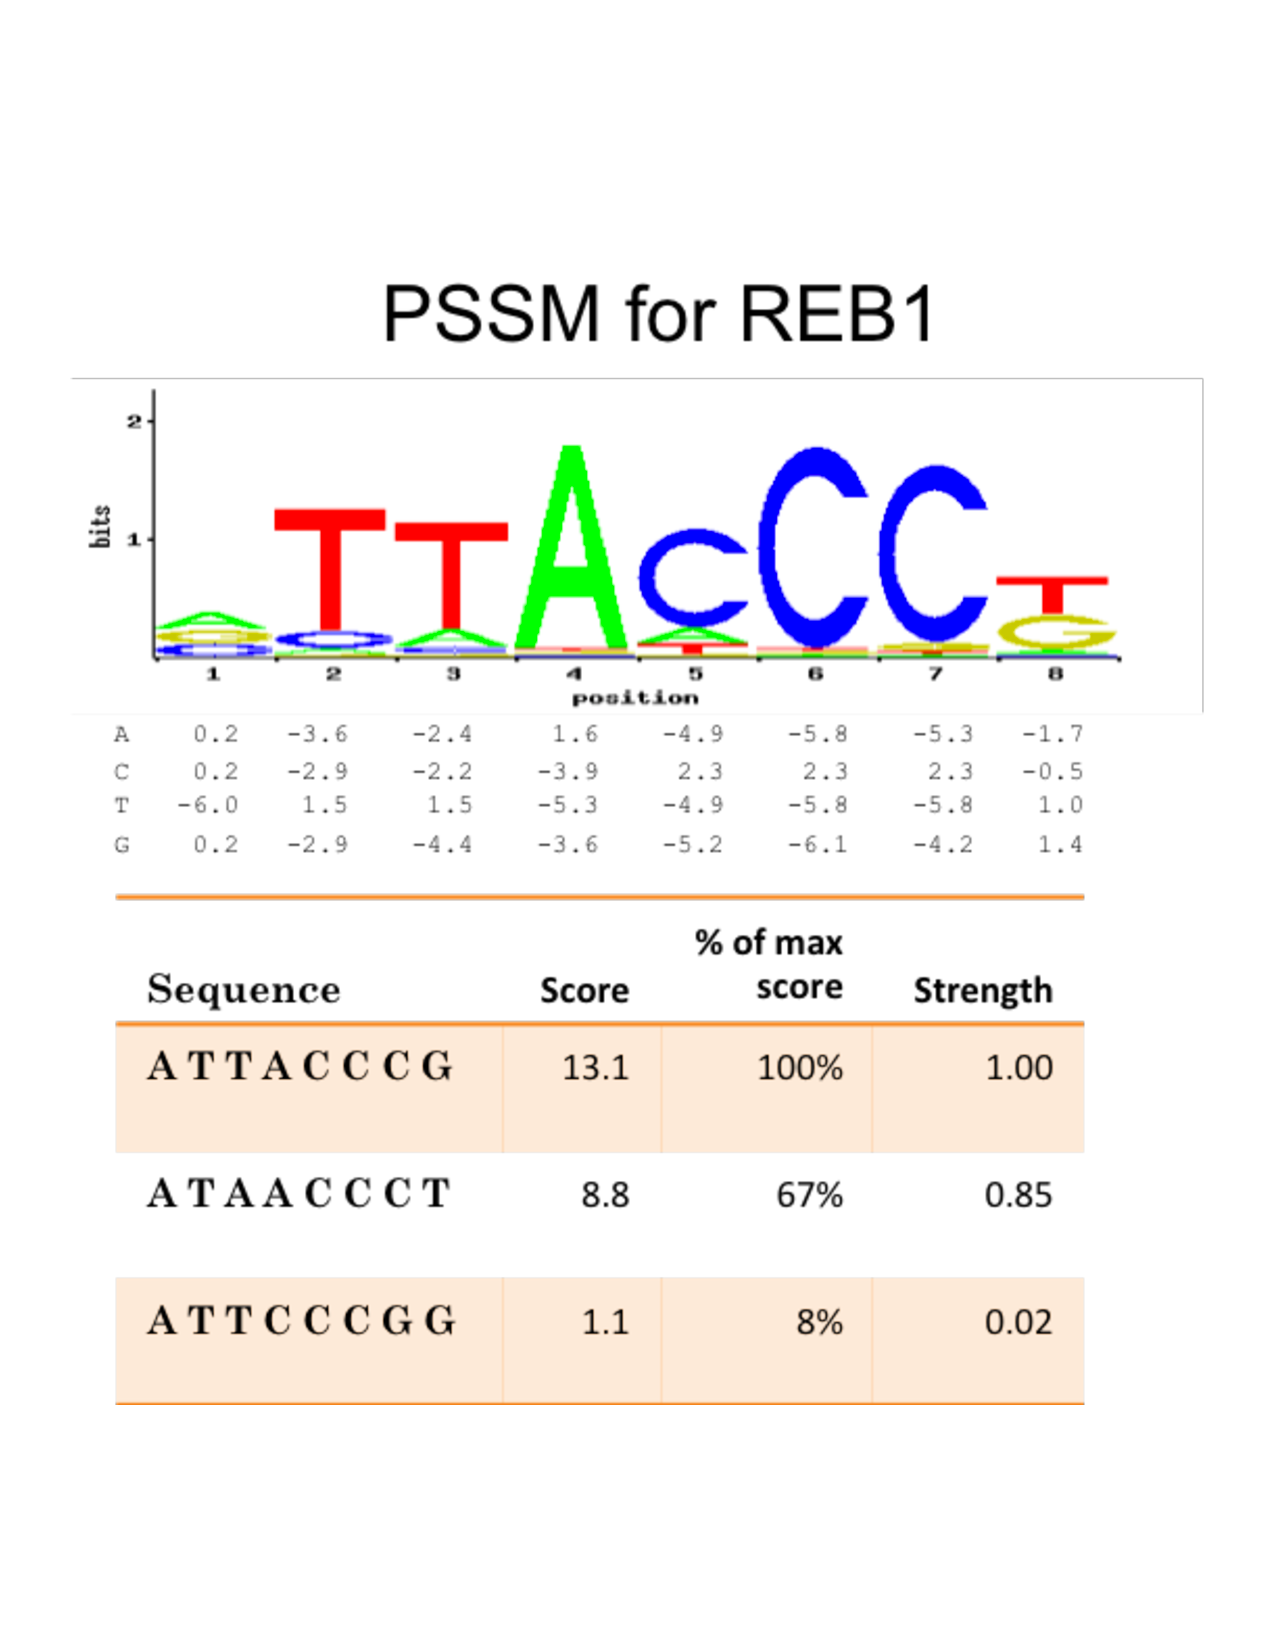
\includegraphics[scale=0.29]{pssm_reb1.pdf}
  \vspace{-11mm}
  \caption{\textbf{TF affinity can be scored for any sequence by using the TFs PSSM.}\\An example PSSM, here for REB1, describes the probability of binding at each nucleotide for any possible sequence. Positions are assumed to be independent and therefore the probability of a TF binding to any arbitrary sequence can be easily calculated.}
  \label{fig:example}
\end{figure}

% \tab The method of converting DNA into RNA, as depicted in Figure \ref{fig:transcriptionprocess}, relies heavily on the process of transcription. Transcription is a process that takes the current DNA state as input and produces an RNA as the output. Biologists are very curious about what happens during the mysterious process of transcription. To study transcription, biologists focus on processes, where DNA, RNA, and proteins are the inputs and outputs of the processes.

% \tab The cycle begins with \textit{transcription}, taking DNA input and producing RNA as the output. Next, \textit{translation} converts the RNA to a set of amino acids that form the protein represented by the DNA. Many of the proteins do not immediately interact with the processes, but are sequestered away from the processing environment, waiting until the cell detects an internal or external \textit{signal} that causes the proteins to return to the processing environment and change its behavior.

% \begin{figure}[H]
%   \centering
%   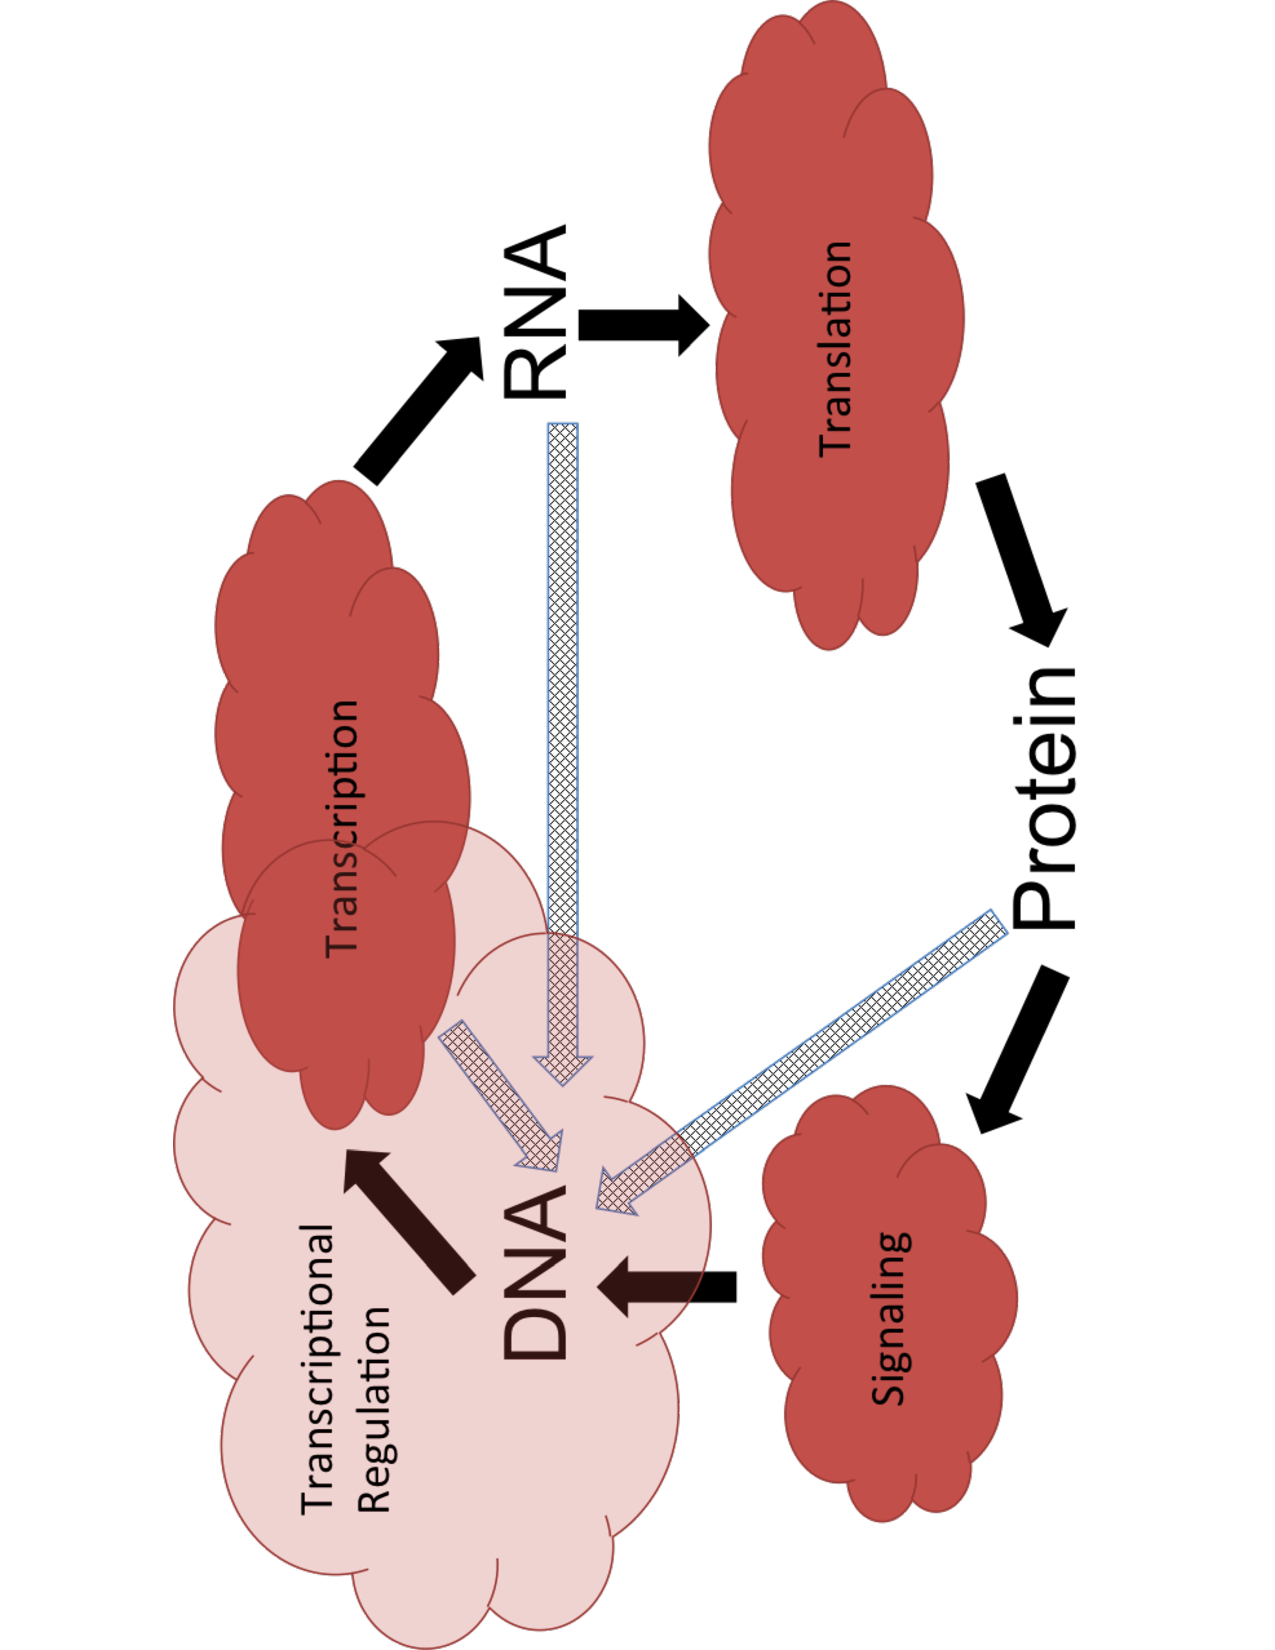
\includegraphics[scale=0.25,angle=270]{transcription_process.pdf}
%   \caption{\textbf{Process of Converting DNA into RNA}}
%   \label{fig:transcriptionprocess}
% \end{figure}

% \tab Current biology textbooks usually show the transcription dogma as a linear process, but we show it as a circular set of processes that feedback upon each other. The processes are shown as clouds and the solid black arrows show the inputs and outputs of the processes. The gray hatched arrows depict the influence on the DNA state by the proteins, the RNA products, and even the transcription process itself.

\section{Methods}

\begin{figure}[H]
  \centering
  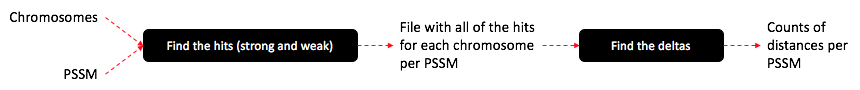
\includegraphics[scale=0.5]{pipeline.png}
  \caption{\textbf{The Approximate Pipeline our Code Follows}}
  \label{fig:pipeline}
\end{figure}

\tab Looking at the pipeline (Figure \ref{fig:pipeline}): we started with a bunch of chromosomes from yeast, $18$ to be exact, in FASTA form, however, we did discarded $2$ of the chromosomes because they didn't give us any useful information. We then took that. Also, we had $124$ transcription factors, with their corresponding PSSMs, in TAMO form. Using this data, we can then take each transcription factor's PSSM and then take each chromosome and calculate all the affinities along the chromosome for that particular transcription factor. Every transcription factor floats around on the chromosome until it finds a match, then after a while, it separates and moves on. Note that when the transcription factor gets to the end of the chromosome, it turns around and goes over the reverse strand (where there could possibly be a match), which is called the "reverse complement" chromosome. Hence, we also run over the reverse complement of each chromosome so that we get a better simulation of what the transcription factor is actually doing. We then take all of these hits and classify them as either \textit{strong} (having a very high affinity chance of the transcription factor binding at that location in the chromosome), \textit{weak} (having a low chance, but still a chance, of binding), or just nothing (when there's close to nothing of a chance of binding). We did output all of these hits (with the corresponding label that we gave them) to GFF (Genetic File Format) files. Please note that the \textit{strong}, \textit{weak}, and nothing classifications have cutoffs. We chose the cutoffs to be $0.75$ or greater is \textit{strong}, $0.35$ and greater until $0.75$ is \textit{weak}, and anything below $0.35$ is classified as nothing.


\tab We wrote another Python program that takes in all of those GFF files, and sees if there are weak spots within some distance (we chose $150$) around each strong spot. The program also plots a histogram of these to show us the frequency of weak binding sites around the strong binding sites.

% \tab Assuming the above, we can then calculate each one of the scores for the entire DNA sequence given each TF. When we do this, we can classify each score as being a strong hit, if it’s greater than our set strong threshold ($0.7$), or a weak hit, if it’s greater than our set weak threshold ($0.35$) but less than our set strong threshold; below the weak threshold, we don’t classify it at all. After we calculate all the hits, we can then analyze them. We do this by going through each strong hit, and for each weak hit, if they happen on the chromosome less than or equal to a certain distance ($150$) away from each other, we add one to a bin that the distance is in. When we’re done, we plot all of the bins in a histogram.

\section{Results}
Unfortunately, since we are dealing with such a big data set, we only ran my code on $30$ different TFs, over all $16$ chromosomes (there were $18$ in the data, but we discarded two of them). Here is an example of a histogram:
\begin{figure}[H]
  \centering
  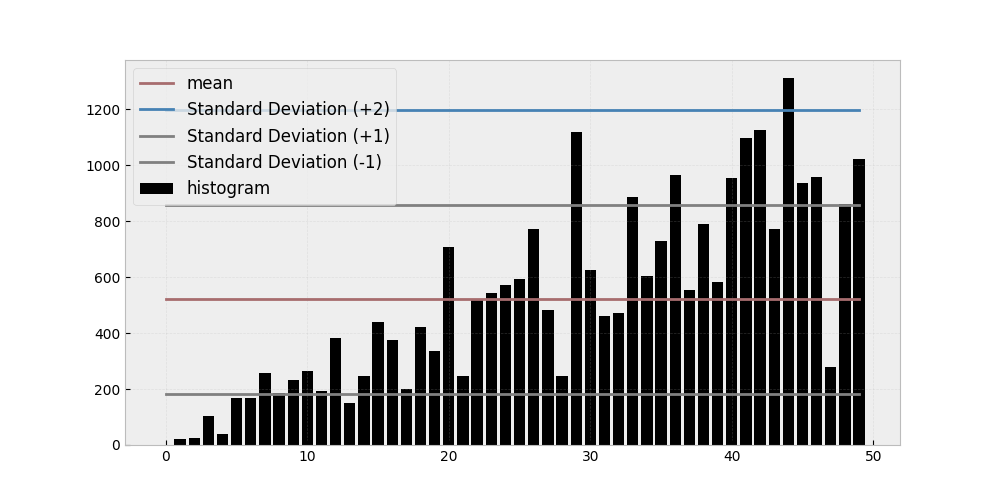
\includegraphics[scale=0.29]{HistGCR1.png}
  \caption{\textbf{Histogram for TF GCR1}}
  \label{fig:histGCR1}
\end{figure}
Please note that this is only a small selection of output histograms that we get. But, the good news is that this is exactly what we were looking for! As you can see from Figure \ref{fig:histGCR1}, there is an overall peak right at $7.5$.
\section{Code}
All the code for this project is hosted on GitHub, located \href{https://github.com/johnletey/PoBT}{here}. Note that we originally started out in MATLAB, but then migrated to Python for efficiency reasons.

\section{Future Work}

As you may have noticed above, we didn't run our code for more than one dataset and also only for one specific settings for parameters. So, in the future we would love to write an overall program to fine tune the parameters that our program uses and test these parameters on different datasets, and see what our program outputs!

\section{Mentions}
\small

\footnotesize{[1] A special thanks to David Knox for the terrific guidance he gave me on the project!}

\footnotesize{[2] Thanks to Matt Shirley for making \href{https://github.com/mdshw5/pyfaidx}{pyfaidx}! It really helped in reading the FASTA data files quickly and efficiently.}

\end{document}